\documentclass[]{article}
\usepackage{url}
\usepackage{graphicx}
%opening
\title{Anomaly Detection in Enron Email Network}
%\author{Volodymyr Miz}

\begin{document}

\maketitle

\begin{abstract}
Anomaly detection in the Enron Email Network.
\end{abstract}

\section{Experiments}
In this experiment, we use the Enron email dataset\footnote{https://www.kaggle.com/wcukierski/enron-email-dataset}. It contains 614586 emails sent over the period from 6 January 1998 until 4 February 2004. During the pre-processing, we remove the periods of low activity and keep the emails from 1 January 1999 until 31 July 2002 which is 1448 days of email records in total. Also, we remove email addresses that sent less than three emails over that period.

To build a graph \mbox{$G = (V,E,W)$}, we use email addresses as nodes $V$. Every node $v_i \in V$ has an attribute which is a time-varying signal that corresponds to the number of emails sent from this address during a day. We draw an edge $e_{ij} \in E$ between two nodes $i$ and $j$ if there is at least one email exchange between the corresponding addresses. Initial weights $W$ are equal to $0$. In total, the initial Enron email network contains 6 600 nodes and 50 897 edges.

In order to detect anomalies in the network activity, we apply the proposed algorithm to the Enron email network and compare our findings to the results presented in\footnote{https://arxiv.org/pdf/1306.0267.pdf}. The authors observe four anomalous periods and relate them to the specific news reports involving Enron. In Figure~\ref{fig: enron}, we show that our algorithm allows detecting all reported anomalies.

In our case, an anomaly is a spike of overall activity in a cluster of email addresses that we detect after learning. The addresses in this cluster cause an anomaly alert since their activity in the network deviates from their common behavior during the considered time period.

\begin{figure}[t!]
	\centering
	%    \captionsetup{justification=centering}
	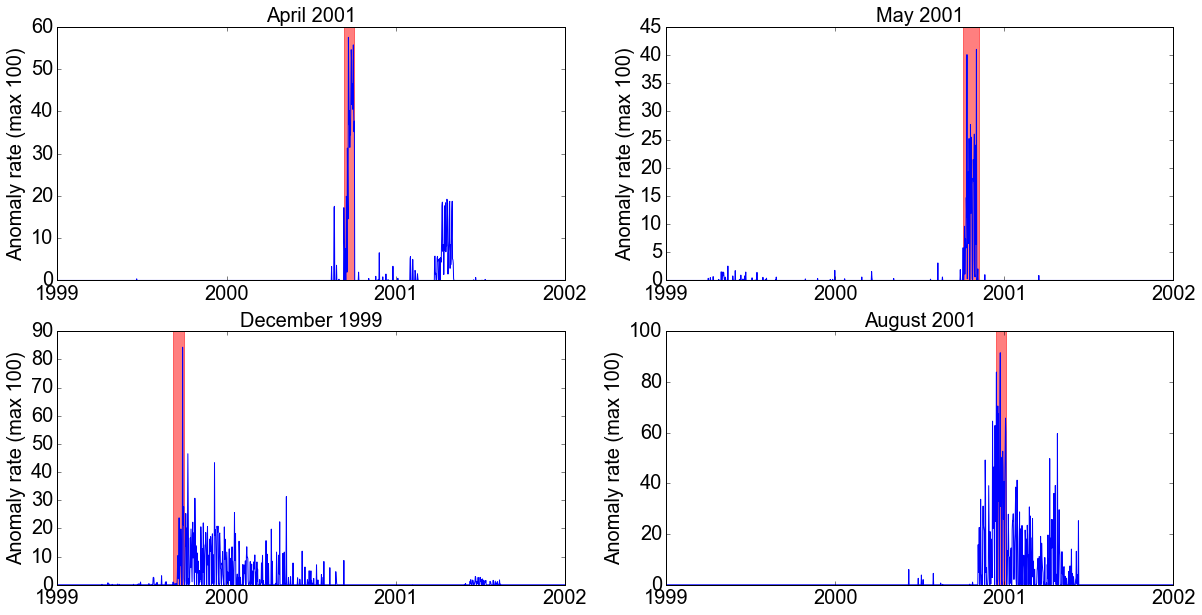
\includegraphics[width=\columnwidth]{figures/enron.png}
	\caption{ Anomaly detection in Enron email network. Red areas highlight the periods previously reported as anomalies (ground truth supported by the real world events). Blue lines reflect the anomaly alert level (scale 0-100) in the network computed by the proposed algorithm.}
	\label{fig: enron}
\end{figure}


\end{document}
